%!TEX root = ../Dokumentation.tex


\section{Entwicklung eines User-Clienten}

\subsection{Vorbereitung und Layoutentwicklung}
Im finalen Meilenstein des Projektes, steht die Entwicklung eines grafischen Userinterface im Mittelpunkt, der die Funktionalität des Systems repräsentiert. Die Applikation soll die entsprechende Verbindung zum Server aufbauen und den Datenaustausch ermöglichen. \\

Vor der praktischen Umsetzung mit Java Swing, wurde ein mögliches Konzeptlayout erstellt und entsprechende Alternativen ausprobiert.Hierbei handelt es sich um erste Ideen wie die Anwendung aufgebaut sein kann und welche Elemente benötigt werden.
Da in der letztendlichen Umsetzung aber hauptsächlich die Funktionalität im Mittelpunkt steht, wurde speziell darauf geachtet, dass alle Funktionalitäten in einem logischen Kontext eingebunden werden und anwendbar sind. Auf genaue Designkonzepte zum optimalen Aufbau wurde hierbei verzichtet, da sie im entsprechenden Projektkontext nicht an erster Stelle stehen sollten. In einem größer angelegten Projekt sollte hierbei eine intensivere Auseinandersetzung folgen mit entsprechender Validierung und Testdurchläufe. \\

Die Applikation soll mit einer Startseite (Abb. 4a) beginnen, von der aus der Anwender die Möglichkeit hat sich zu identifizieren. Entweder er meldet sich mit bereits vorhandenen Daten an oder er registriert sich als neuer Benutzer.
Sind bereits Accountdaten vorhanden, so folgt eine Eingabe des Usernamen und des Passworts (Abb. 4b). Sollte der User eine der beiden Informationen vergessen haben, so besteht die Option \textit{Passwort/Username vergessen?}, wobei die funktionale Implementierung nicht stattfinden wird und dies eher als Platzhalter dient. Nach Eingabe der Daten und Prüfung auf Korrektheit, wird zur \textit{Homeseite} weitergeleitet, die als Hauptseite dient und von der aus die verschiedenen Funktionen angesteuert werden.

\begin{figure}[h!]
\centering
\hfill %
\subfloat[Startseite \label{pic:Anmelden}]{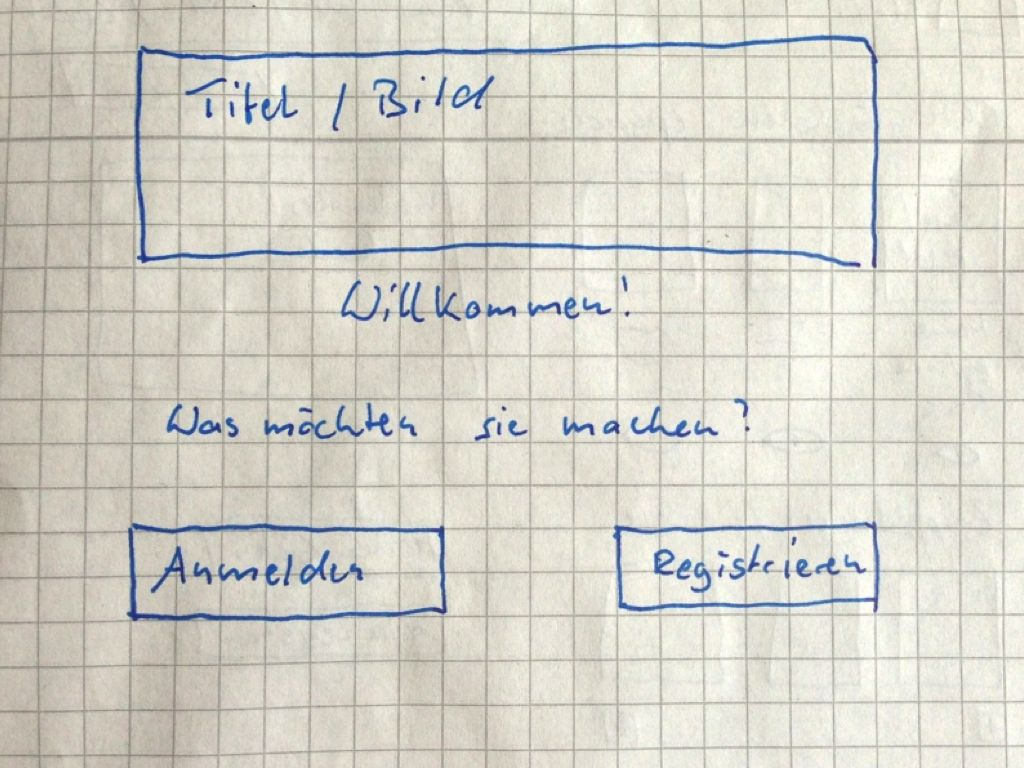
\includegraphics[width=.5\textwidth]{../images/dokulayout/startseite.jpg}}
\hfill % alternativ auch \hspace{1cm} für genaue Angaben
\subfloat[Einloggen \label{pic:Registrieren}]{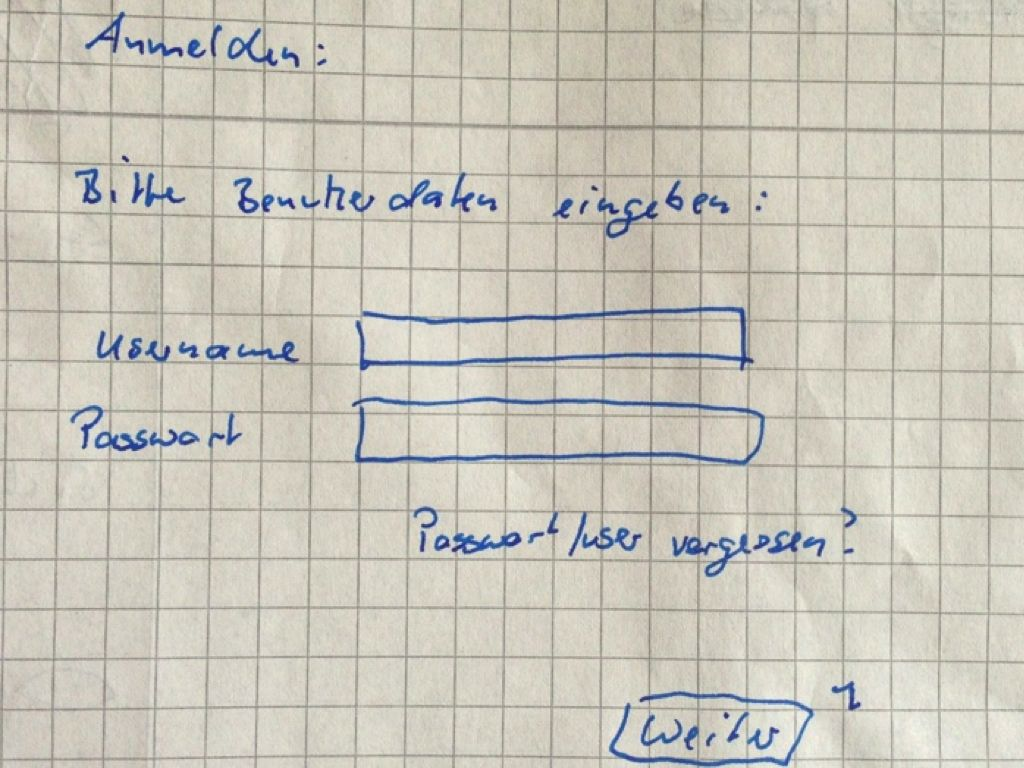
\includegraphics[width=.5\textwidth]{../images/dokulayout/anmelden.jpg}}
\hfill %
\caption{Gui Layout Skizzen: Startauswahl und Einloggen }
\label{Gui}
\end{figure}




\newpage

Entscheidet man sich für die Auswahl \textit{Registrieren} wird ein neuer Account angelegt. Auf der ersten Seite (Abb. 5a) werden die Grundinformationen eingegeben, wobei hier nur Username und Passwort und Name notwendig sind und die zusätzlichen Informationen jederzeit ergänzt werden können. Nach Eingabe und Kontrolle folgt der zweite Teil der Registrierung, die Auswahl der Genreprioritäten (Abb. 5b). Da der Serientracker die Option anbietet, Informationen zu Serien eines bestimtmen Genres zu erhalten, dient dieser Schritt dazu bestimmte Genres zu abonnieren. Auch hier soll die Auswahl später geändert werden können.\\

\begin{figure}[h!]
\centering
\hfill
\subfloat[Registrieren \label{pic:Registrieren}]{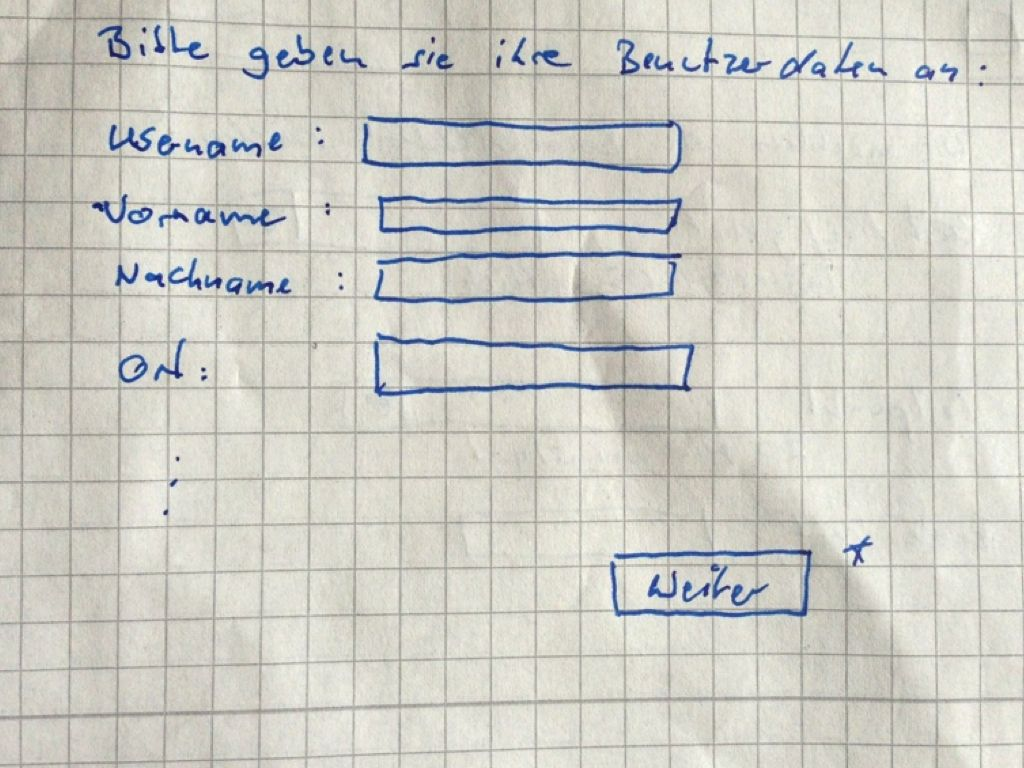
\includegraphics[width=.5\textwidth]{../images/dokulayout/registrieren.jpg}}
\hfill % alternativ auch \hspace{1cm} für genaue Angaben
\subfloat[Prioritäten \label{pic:Prioritaeten}]{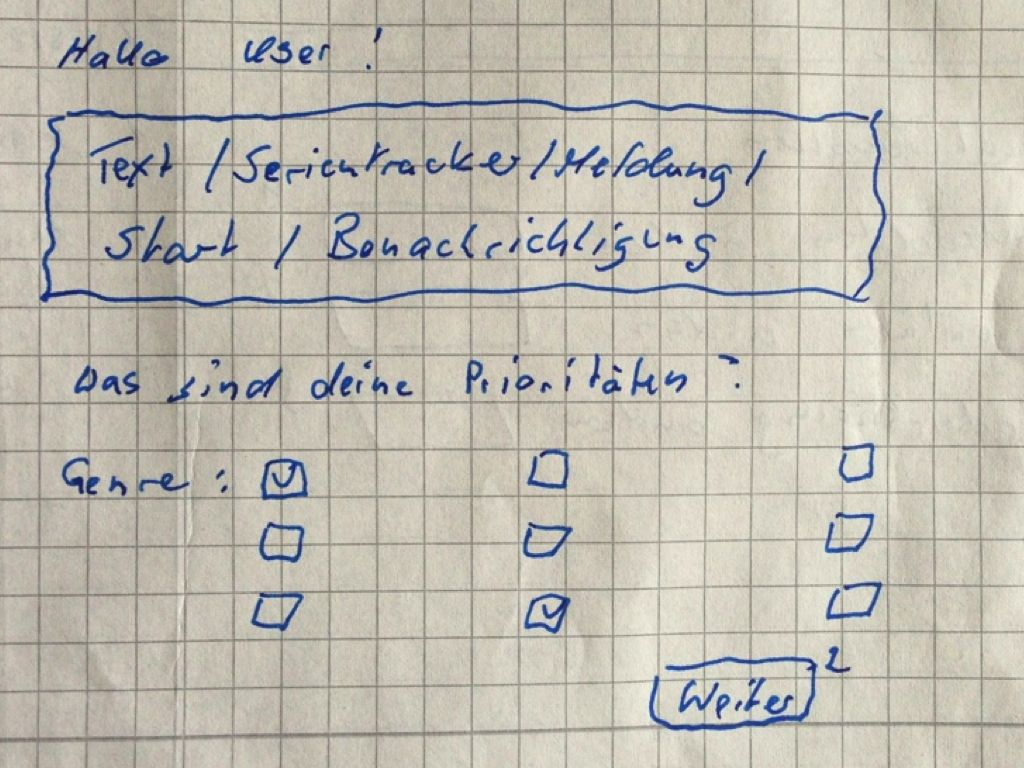
\includegraphics[width=.5\textwidth]{../images/dokulayout/prioritaeten.jpg}}
\hfill %
\caption{Gui Layout Skizzen: Registrierung }
\label{Gui}
\end{figure}

\parskip 12pt
\parindent 0pt


\begin{wrapfigure}{r}{0cm}
\centering
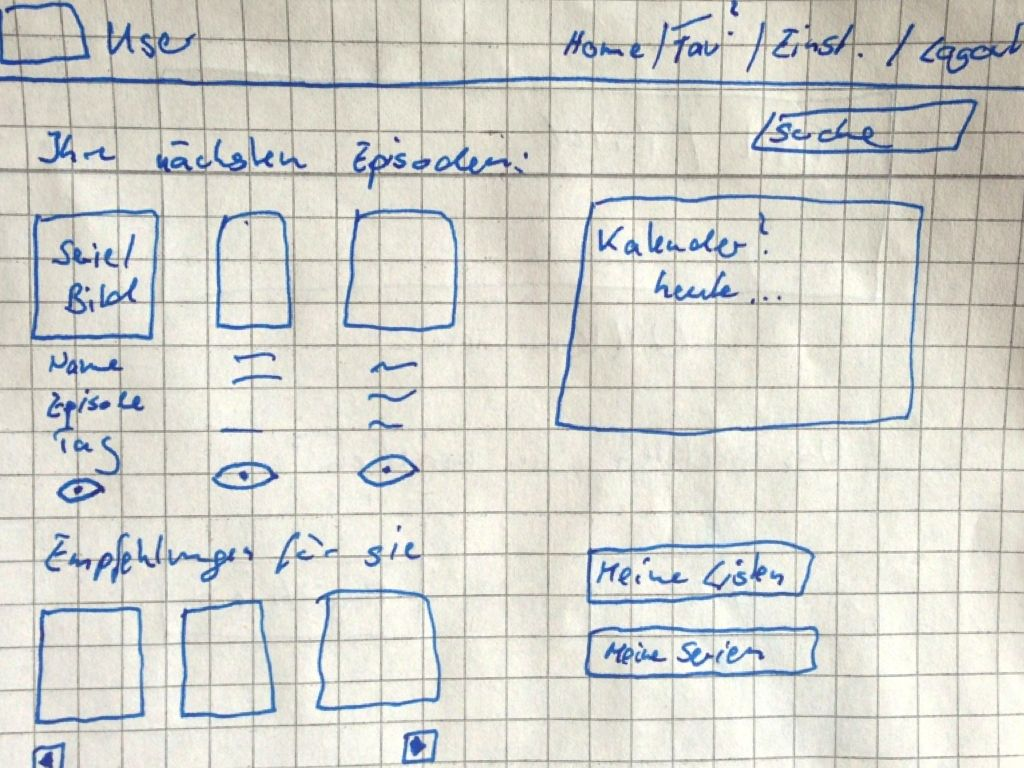
\includegraphics[width=.5\textwidth]{../images/dokulayout/home.jpg}
\caption{Gui Skizzen: Homeansicht}
\end{wrapfigure}

Nach erfolgreicher Identifizierung des Users folgt der Homebereich (Abb. 6). Dies ist der eigentliche Ausgangspunkt für alle Aktivitäten und dient als Benutzerzentrale. Am oberen Bereich findet sich eine statische Menüleiste, die sich in diesem Aufbau durch alle weiteren Bereiche zieht und jederzeit zugänglich ist. Information zum angemeldeten User und die Optionen \textit{Home}, \textit{Favoriten}, \textit{Einstellung}und\textit {Logout}. Home führt jederzeite zur Hauptübersicht, Einstellung ermöglicht entsprechende Möglichkeiten zur Accountverwaltung und Logout meldet den aktuellen Benutzer ab und führt wieder zur Anmeldung. Die Option Favoriten war als Verwaltung zu den angelegten Lieblingsgenre geplant, wurde aber in weiteren Entwürfen in die Einstellungen mit eingebunden, da bis auf eine einfache Auswahl kein größerer Nutzen für den User angeboten wird. Für den Fall das Adminrechte vorhanden sind, wurde in einem späteren Entwurf der zusätzliche Menüpunkt \textit{Hinzufügen} eingebunden. Dort lassen sich neue Serien, Staffeln, Episoden und Genrelisten anlegen. \\


\newpage

Da im Mittelpunkt des Konzeptes die Benachrichtigung über neue Episoden steht, werden dem User bereits nach einloggen die wichtigsten Informationen präsentiert. Neben einer Suche, werden die Ausstrahlungszeitpunkte der nächsten Episoden angezeigt. Neben dieser Übersicht sollten zudem direkte Benachrichtigungen in Form von Pop-Ups stattfinden, weshalb diese Ansicht vorallem der Erinnerung und Verwaltung dient. Inwiefern eine Darstellung der heutigen Serien in Form eines Kalender realisierbar wäre ist zur Zeit der Konzipierung noch unklar, sollte aber eher als \textit{nice-to-have Feature} betrachtet werden.\\
Dazu gab es die Überlegung Serienempfehlung zu geben, basiernd auf abonnierten Genres. Buttons zu \textit{Meine Serien} und \textit{Meine Listen} führen zu entsprechenden Unterkategoerien.
Meine Serien zeigt einer Auflistung der Serien über die man Benachrichtigungen erhalten möchte und die derzeit angeschaut werden. Meine Listen gibt einen Überblick über angelegte Listen zur Ordnung von Serien nach bestimmten Themen und bietet zudem die Möglichkeit eine neue Liste anzulegen. \\

\parskip 12pt
\parindent 0pt

Nach Auswahl einer bestimmten Serie werden vorhandene Information präsentiert. Allgemeine Informationen, eine Übersicht zu vorhandenen Staffeln und eine Darstellung der nächsten Episode die Ausgestrahlt wird und gegebenfalls die Episode die der Benuter zuletzt gesehen hat. Hierbei würde die Verwaltung mit Hilfe der Seen List stattfinden, wobei auch hier die letztendliche Umsetzung eher unwahrscheinlich ist.
Auf dieser Seite (Abb. 7a) kann die Serie einer bestimmten Liste hinzugefügt werden und wird damit abonniert. In einer weiteren Variante der Serienseite (Abb. 7b) handelt es sich um die Darstellung unter Adminrechte, wobei die \textit{Add to List} Option nun zum Editieren dieser Seite führt und auch neben den Serien eine entsprechende Editierfunktion eingeführt wird.

\begin{figure} [h!]
\centering
\hfill %
\subfloat[Serienseite User \label{pic:Serienseite}]{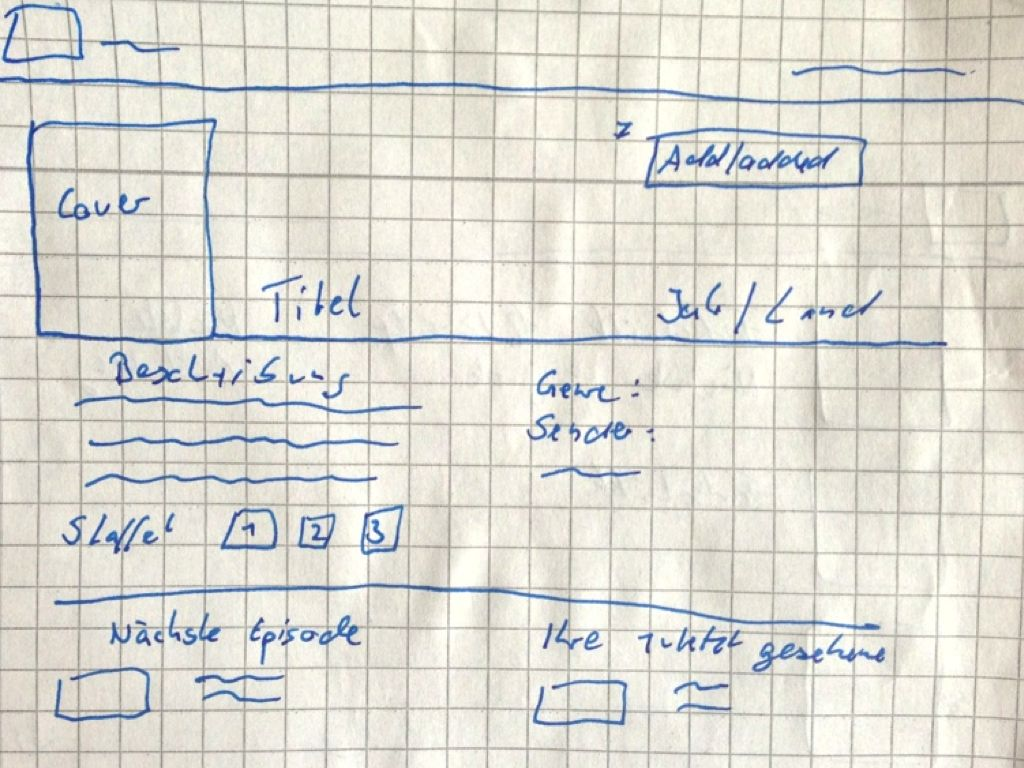
\includegraphics[width=.5\textwidth]{../images/dokulayout/serie.jpg}}
\hfill % alternativ auch \hspace{1cm} für genaue Angaben
\subfloat[Serienseite Admin \label{pic:Serienseite}]{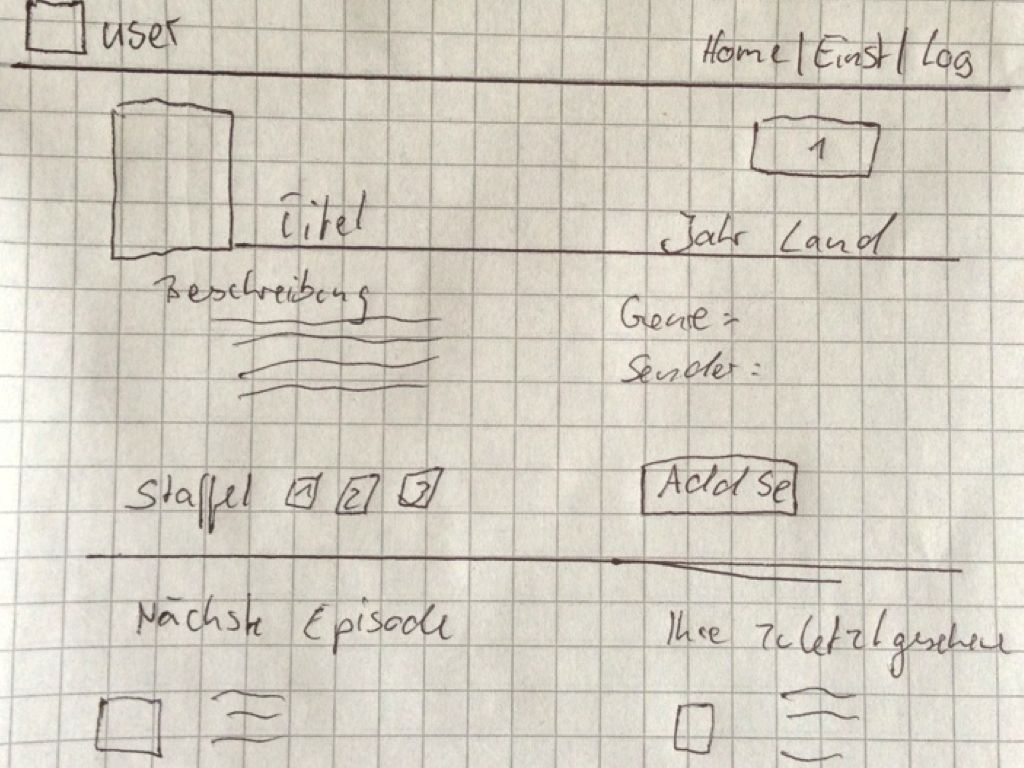
\includegraphics[width=.5\textwidth]{../images/dokulayout/serie2.jpg}}
\hfill %
\caption{Gui Layout Skizzen: Serienübersicht }
\label{Gui}
\end{figure}


\newpage

Die jeweilige Seasonseite (Abb. 8a) zeigt eine Vorschau zu vorhandenen Episoden und bietet dem Admin erneut die \textit{Add Episode} Funktion (Abb. 8b). In welcher Form die Episoden aufgeführt werden ist zu diesem Zeitpunkt noch nicht festgelegt und wird bei entsprechender Umsetzung entschieden. Wird eine neue Episode angelegt (Abb. 8b) wird entsprechende Serie und Staffel referenziert und die einzelnrn Informationen eingegeben.\\
\begin{figure} [h!]
\centering
\hfill %
\subfloat[Seasonseite \label{pic:Seasonseite}]{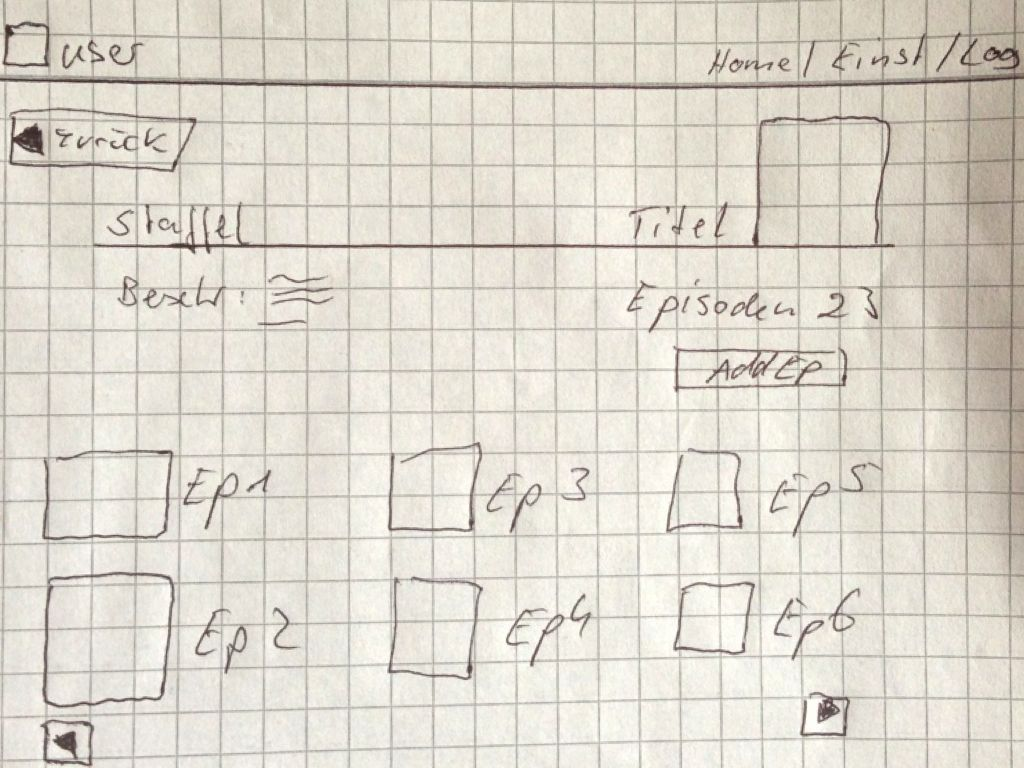
\includegraphics[width=.5\textwidth]{../images/dokulayout/staffel.jpg}}
\hfill % alternativ auch \hspace{1cm} für genaue Angaben
\subfloat[Episode anlegen \label{pic:Episodenverwaltung}]{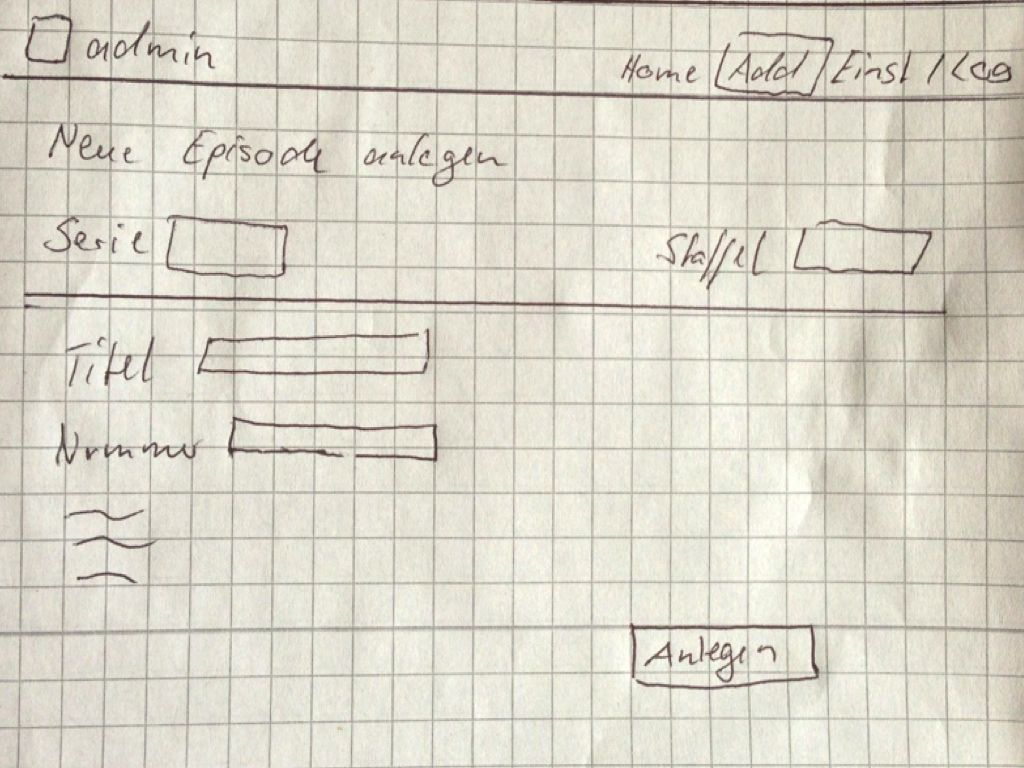
\includegraphics[width=.5\textwidth]{../images/dokulayout/anlegen.jpg}}
\hfill %
\caption{Gui Layout Skizzen: Seasonübersicht und Verwaltung }
\label{Gui}
\end{figure}

Bei der Planung der GUI, wurden die einzelnen Seiten nach entsprechenden Ideen konzipiert und weiterentwickelt. Die vorgestellten Entwürfe sollten einen kurzen Einblick in die Planungsphase geben und dienten in dieser Form keiner finalen Vorlage, nach der die Entwicklung stattfindet. Aus diesem Grund wird hier im weiteren nicht auf jede einzelne Unterseite eingegangen.\\ Während bei den ersten Varianten vorallem der mögliche Aufbau und die Darstellung der einzelnen Elemente im Vordergrund stand, wurden in späteren Versionen speziell auf entsprechende Funktionalität und Verweisen geachtet. Dabei entstand unter anderem die Adminansicht, welche die Kategorien um verwaltende Optionen erweitert. Ob jede Vorstellung realisierbar bzw. im Projektkontext notwendig ist und wie sich entsprechendes Layout letztendlich entwickelt hat, wird in der Umsetzung dargestellt. (Diesen Absatz eventuell überarbeiten, noch nicht ganz passend) \\

\newpage
\subsubsection{Umsetzung}
